%%%%%%%%%%%%%%%%%%%%%%%%%%%%%%%%%%%%%%%%%%%%%%%%%%%%%%%%%%%%
%
% Authors:       Nina Wiedemann, Benjamin Ummenhofer, Diana Wofk, 
%                Quentin Leboutet, and Michael Paulitsch
%
% Description:   The SYCL of Life: Evolutionary Kernel Optimization 
%                with Large Language Models
%
% Section:       Method
%
%%%%%%%%%%%%%%%%%%%%%%%%%%%%%%%%%%%%%%%%%%%%%%%%%%%%%%%%%%%%


\section{Method} \label{sec:method}


\subsection{System Architecture} \label{sec:architecture}

% \vspace{-3mm}
\begin{figure}[t!]
	\centering
    \resizebox{0.6\linewidth}{!}{\PipelineDiagramB}
	\caption{The KernelFoundry pipeline: evolutionary kernel optimization with multi-level feedback and meta-prompt co-evolution.}
	\label{fig:pipeline}
	\vspace{-3mm}
\end{figure}

We present KernelFoundry, an evolutionary framework for LLM-driven GPU kernel optimization. Figure~\ref{fig:pipeline} illustrates the architecture, which comprises five tightly-coupled components. The process begins with a \textbf{task specification layer} that accepts kernel generation problems in a flexible format  supporting PyTorch reference implementations, high-level natural language descriptions, or existing kernels requiring optimization. The system natively supports KernelBench~\citep{ouyang2025kernelbench} tasks as well as custom workloads with user-defined test frameworks. A \textbf{prompt construction engine} then assembles context-aware prompts by combining the task specification with hardware-specific optimization guidance, sampled parent programs and inspirations from the archive, gradient-derived mutation hints, and dynamically evolved prompt components (\S\ref{sec:metaprompting}). The resulting prompt is served to an \textbf{LLM inference backend}, which provides a unified interface to both API-based models (OpenAI, Anthropic) and locally-hosted models via vLLM, and generates multiple candidate kernels. Candidates are processed by a \textbf{compilation \& evaluation pipeline} that compiles to the target backend (SYCL via Intel DPC++, CUDA via nvcc, or Triton), validates numerical correctness against reference implementations, measures execution time, and optionally collects profiling data via Intel \emph{unitrace} or NVIDIA \emph{Nsight}. Finally, an \textbf{evolutionary archive} implements MAP-Elites~\citep{mouret2015illuminating} by organizing kernels according to behavioral coordinates in an optimization feature space (\S\ref{sec:mapelites}). It retains the best-performing kernel (elite) for each occupied cell, thereby preserving diversity across qualitatively different optimization strategies.
In similar spirit, we evolve sections of the prompt with \textbf{meta-prompt evolution} which maintains a separate archive with successful guidance examples.\\
The evolutionary loop proceeds as follows. At each iteration, parent programs are sampled from the archive using selection strategies informed by fitness, exploration potential, and gradient estimates. The prompt constructor assembles a generation prompt incorporating parent code, feedback from prior evaluations, and optimization guidance. 
The LLM generates candidate kernels, which undergo compilation, correctness testing, and performance measurement. Candidates that run correctly are assigned behavioral coordinates via static code analysis; those improving upon existing elites are inserted into the archive. Feedback from all outcomes (including failures) informs subsequent iterations through the gradient estimator and meta-prompter.

\subsection{Quality-Diversity Search with MAP-Elites} \label{sec:mapelites}
Standard evolutionary approaches optimize a single objective (e.g., runtime), risking convergence to local optima without exploring alternative solution strategies. Quality-Diversity (QD) algorithms~\citep{pugh2016quality} address this limitation by maintaining diverse collections of high-performing solutions in independent behavioral cells, enabling discovery of stepping-stone solutions that facilitate escape from local optima.


% \vspace{-3mm}

\paragraph{MAP-Elites Algorithm.}
MAP-Elites~\citep{mouret2015illuminating} partitions the solution space into a discrete grid based on \textit{behavioral descriptors} which are low-dimensional features characterizing solution behavior independent of fitness. Each cell maintains the highest-fitness solution discovered for that behavioral region. The algorithm iterates in four phases (\textbf{selection}, \textbf{variation}, \textbf{evaluation}, and \textbf{insertion}). During \textbf{selection}, the system samples parent kernel(s) from the archive using a configurable strategy (uniform, fitness-proportionate, curiosity-driven, or island-based). During \textbf{variation}, it produces offspring via LLM-based code modification guided by the parent kernel, optimization hints, and meta-evolved prompt content. During \textbf{evaluation}, the offspring is compiled, validated for correctness, benchmarked for performance, and assigned behavioral coordinates via static code analysis. During \textbf{insertion}, the offspring replaces the incumbent elite if it improves upon the existing elite (or if the target cell is empty); otherwise it is discarded.
This mechanism maintains diversity by construction: the archive cannot collapse because each cell evolves independently.
\begin{figure*}[t]
\centering
    % \vspace{-3mm}
	% \MAPElitesGridCorrected{$d_\text{mem}$}{$d_\text{algo}$}{$d_\text{sync}$}{4}{4}{4}{42}
    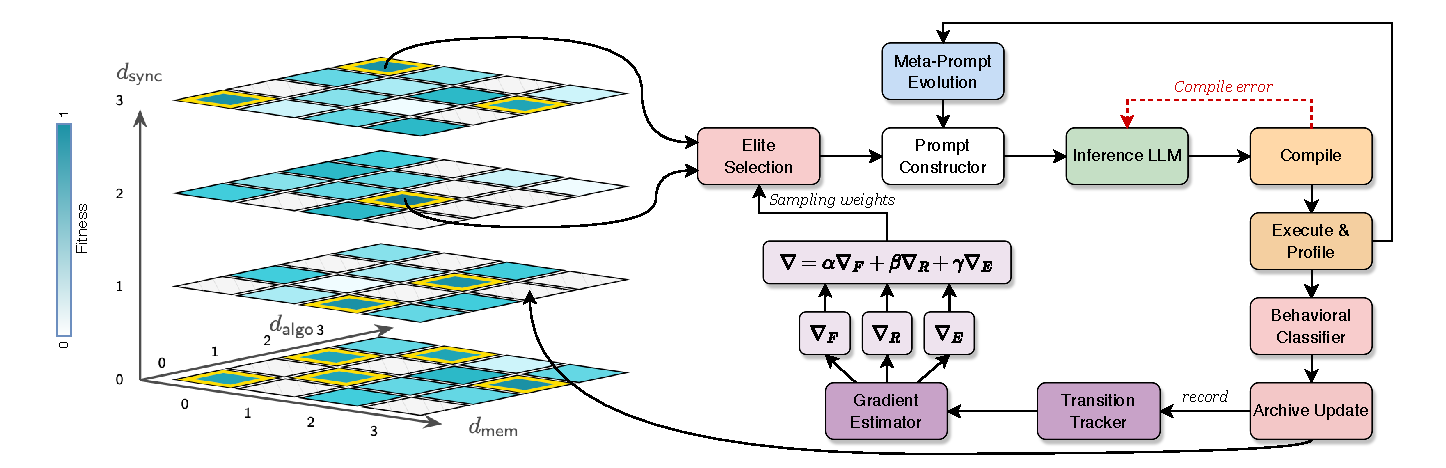
\includegraphics[width=\textwidth]{Figures/MAPEliteGrid.drawio.pdf}
    % \vspace{-6mm}
    \caption{Gradient-informed MAP-Elites for kernel optimization. The archive partitions kernels by behavioral coordinates $(d_\text{mem}, d_\text{algo}, d_\text{sync})$. Elites are shown in yellow. A Transition Tracker records parent$\to$child transitions with behavioral coordinates and fitness deltas. The Gradient Estimator combines fitness gradients ($\nabla F$), improvement-rate gradients ($\nabla R$), and exploration gradients ($\nabla E$) to produce sampling weights and natural-language mutation hints that guide subsequent generations.}
    % \end{minipage}
	\label{fig:qd-mapelites0}
    % \vspace{-3mm}
\end{figure*}

\vspace{-3mm}


\paragraph{Kernel-Specific Behavioral Descriptors.}
Adapting the MAP-Elites algorithm to kernel optimization requires defining behavioral descriptors that capture meaningful optimization characteristics. With KernelFoundry, we propose a three-dimensional optimization feature space with discrete levels reflecting increasingly sophisticated optimization patterns. These coordinates are computed deterministically from generated code via static pattern matching on SYCL and CUDA constructs, ensuring reproducibility and reducing execution-time variability.

\begin{enumerate}[leftmargin=1.5em,itemsep=0pt]
    \item \textbf{Memory Access Pattern} ($d_\text{mem} \in \{0,1,2,3\}$):
    \begin{description}[leftmargin=*,itemsep=0pt,labelsep=1mm]
        \item[0:] Scalar, strided, or uncoalesced access
        \item[1:] Coalesced/vectorized (vec4, aligned loads)
        \item[2:] Shared/local memory with explicit tiling
        \item[3:] Multi-level\ hierarchy (SLM + reg.\ blocking + prefetch)
    \end{description}
    
    \item \textbf{Algorithmic Structure} ($d_\text{algo} \in \{0,1,2,3\}$):
    \begin{description}[leftmargin=*,itemsep=0pt,labelsep=1mm]
        \item[0:] Direct PyTorch translation 
        \item[1:] Fused operations (single-pass over data)
        \item[2:] Reformulated algorithm (online norm., flash pattern)
        \item[3:] Novel/asymptotically improved algorithm
    \end{description}
    \item \textbf{Parallelism Coordination} ($d_\text{sync} \in \{0,1,2,3\}$):
    \begin{description}[leftmargin=*,itemsep=0pt,labelsep=1mm]
        \item[0:] No synchronization (embarrassingly parallel)
        \item[1:] Work-group barriers (\texttt{group::barrier})
        \item[2:] Sub-group primitives (shuffles, reductions, broadc.)%broadcasts)
        \item[3:] Global coordination (atomics, multi-pass with sync)
    \end{description}

\end{enumerate}
This three-dimensional grid yields $4^3 = 64$ behavioral cells. 
The classifier employs weighted pattern matching with category-specific patterns to avoid double-counting related constructs (e.g., a kernel using \emph{group\_barrier} for SLM synchronization receives credit in $d_\text{mem}$ for SLM usage, not additionally in $d_\text{sync}$ for the same barrier).


\paragraph{Fitness Function.}
The fitness function prioritizes correctness while rewarding performance:
% \vspace{-2mm}
\begin{equation*}
f(k)=
\begin{cases}
0 & \text{if compilation fails}, \\
0.1 &  \text{if compiles but incorrect}, \\
0.5+0.5 \cdot s_{\text{norm}} &  \text{if correct},
\end{cases}
% \vspace{-2mm}
\end{equation*}
where $s_{\text{norm}} = \min(1, \text{speedup} / \text{target})$ is the normalized speedup relative to a configurable target (default: $2\times$ over PyTorch baseline). This design ensures that correctness is a prerequisite for high fitness while providing a continuous gradient for performance optimization.

% \vspace{-3mm}

\paragraph{Selection Strategies.}
We implement four parent selection strategies, with configurable mixing ratios:
\vspace{-0.5em}
\begin{itemize}[leftmargin=2em,itemsep=0pt]
    \item Uniform selection samples randomly from occupied cells to maximize behavioral diversity. 
    \item Fitness-proportionate selection weights sampling by elite fitness to exploit high-performing regions. 
    \item Curiosity-driven selection prioritizes cells with high estimated improvement potential as inferred from the gradient signal.
    \item Island-based selection maintains $K$ independent sub-populations with periodic migration every $M$ generations, balancing isolated exploration with cross-pollination.
\end{itemize}


\subsection{Gradient-Informed Evolution} \label{sec:gradient}

While the archive structure prevents global mode collapse, individual cells may stagnate if the LLM repeatedly produces similar variants. Inspired by CMA-ME~\citep{cmame} and PGA-MAP-Elites~\citep{pgamapelites}, we augment MAP-Elites with gradient-like signals derived from evolutionary transition history. These gradients provide a \textit{soft steering mechanism} that complements the archive's structural diversity guarantees.

% \vspace{-3mm}

\paragraph{Transition Tracking and gradient estimation.}
We maintain a circular buffer of recent parent$\to$child transitions. Each transition record stores the parent and child behavioral coordinates $(\mathbf{b}_p, \mathbf{b}_c)$, the fitness delta $\Delta f = f_c - f_p$, the transition outcome (\textcolor{green!60!black}{improvement} when the child becomes an elite or discovers a new cell, \textcolor{gray}{neutral} when it is competitive but does not update the archive, or \textcolor{red!70!black}{regression} when fitness decreases), as well as a timestamp and iteration number for temporal weighting.\\
% Per-cell statistics aggregate incoming and outgoing transitions, tracking improvement rates and average fitness changes for each transition direction.
%
%\vspace{-3mm}
%
%\paragraph{Gradient Estimation.}
From the accumulated transitions, we compute three gradient components for each occupied cell~$\mathbf{b}$. The \textit{Fitness gradient} $\nabla_\mathbf{b} F$ estimates which directions in behavioral space improve fitness. For each dimension $d$, we aggregate transitions weighted by fitness delta and direction:
\begin{equation}
    \nabla_d F \approx \frac{1}{|\mathcal{T}|} \sum_{t \in \mathcal{T}} \Delta f_t \cdot \text{sign}(b_c^{(d)} - b_p^{(d)}) \cdot w(t)
\end{equation}
where $\mathcal{T}$ is the set of transitions originating from cell $\mathbf{b}$, and $w(t)$ applies exponential time decay to prioritize recent experience.
\textit{Improvement-rate gradient} $\nabla_\mathbf{b} R$ estimates which directions yield higher improvement probability, independent of improvement magnitude:
\begin{equation}
    \nabla_d R \approx P(\text{imp.} \mid \Delta b_d > 0) - P(\text{imp.} \mid \Delta b_d < 0)
\end{equation}
\textit{Exploration gradient} $\nabla_\mathbf{b} E$ points to empty or low-quality cells, weighted by inverse distance and improvement potential:
\begin{equation}
    \nabla_\mathbf{b} E \propto \sum_{c \in \mathcal{E}} \frac{(f_{\max} - f_c)}{\|\mathbf{c} - \mathbf{b}\|_1} \cdot \frac{\mathbf{c} - \mathbf{b}}{\|\mathbf{c} - \mathbf{b}\|_1}
\end{equation}
where $\mathcal{E}$ is the set of empty cells and low-quality occupied cells.
The combined gradient is a weighted average, 
\begin{equation}
\nabla_\mathbf{b} = \alpha \nabla F + \beta \nabla R + \gamma \nabla E,\, \text{with} (\alpha, \beta, \gamma) = (0.4, 0.4, 0.2).
\end{equation}
% \vspace{-3mm}
\paragraph{Gradient-to-Prompt Translation.}
Gradients inform the optimization process at two levels. For \textit{parent selection}, cells with strong positive gradient magnitudes receive higher sampling probability, directing computational effort toward productive regions. For \textit{prompt construction}, gradient directions are translated into natural-language mutation hints. For example, a positive gradient in $d_\text{mem}$ yields hints such as ``\textit{consider adding shared memory tiling}'' or ``\textit{implement register blocking for data reuse}.'' These hints are injected into the generation prompt, providing actionable guidance grounded in empirical transition success.


\subsection{Templated Kernels for Parameter Tuning} \label{sec:templated}

Beyond algorithmic transformations, kernel performance depends critically on hardware-specific parameters such as work-group dimensions, tile sizes, and unroll factors. Rather than requiring the LLM to guess optimal values, we enable explicit parameter exploration through templated kernel generation.
The prompt instructs the LLM to optionally produce a \textit{templated kernel} with configurable parameters alongside a dispatch function enumerating valid parameter combinations. 
Our evaluation pipeline detects templated kernels, extracts parameter configurations,
% from the dispatch function,
and evaluates each instantiation independently. The best-performing configuration determines the kernel's fitness, while all results are logged to enable the LLM to refine parameter choices in subsequent iterations. This approach separates algorithmic optimization from parameter tuning, allowing the evolutionary search to explore both dimensions efficiently.

% \subsection{Meta-Prompting: Counteracting Context Degradation} \label{sec:metaprompting}

% \vspace{-1mm}
\subsection{Meta-Prompting Against Context Degradation} \label{sec:metaprompting}

As evolutionary search progresses, accumulated experiment histories can degrade generation quality as failed attempts dominate the context: a phenomenon termed \textit{context pollution}~\citep{yan2026pacevolve}. %Successful discoveries are inherently sparse; failed attempts dominate the context, biasing the model toward previously unsuccessful directions. 
Inspired by CodeEvolve~\citep{codeevolve} and GEPA~\citep{gepa}, we introduce \textbf{meta-prompt evolution}: prompts are mutable and co-evolve with kernels, enabling successful optimization strategies to propagate while unsuccessful guidance is pruned.

% \vspace{-3mm}

\paragraph{Evolvable Prompt Regions.}
The kernel generation prompt contains four evolvable sections, delimited by special markers. Specifically, we evolve (1) \textbf{optimization philosophy}, which encodes high-level principles that shape priorities (e.g., ``\textit{prioritize memory bandwidth utilization before compute optimization}''), (2) \textbf{optimization strategies}, which enumerate concrete techniques organized by category (memory, compute, parallelism) together with canonical code patterns and short explanations, (3) \textbf{common pitfalls}, which list anti-patterns and frequent mistakes to avoid (e.g., ``\textit{avoid bank conflicts by adding padding to shared memory arrays}''), and (4) \textbf{analysis guidance}, which provides a pre-coding reasoning scaffold that prompts the LLM to identify likely bottlenecks before generating code.

% \vspace{-3mm}

\paragraph{Meta-Prompter LLM.}
This dedicated LLM (distinct from the kernel generator) analyzes generation outcomes and proposes prompt modifications. Given the current evolvable prompt sections together with the generated kernel code and evaluation metrics (correctness, speedup, and error messages), the meta-prompter first diagnoses which guidance was missing, misleading, or insufficiently specific for the observed outcome. It then prescribes targeted updates as SEARCH/REPLACE diffs restricted to the evolvable regions.
This two-LLM architecture separates analysis from generation, allowing the meta-prompter to specialize in prompt refinement without conflating it with kernel synthesis.

% \vspace{-3mm}

\paragraph{Prompt Archive and Co-Evolution.}
Evolved prompts are maintained in their own archive, with fitness defined by the best kernel performance achieved using each prompt variant. 
Kernels and prompts co-evolve in an interleaved schedule: every $N$ kernel generations (default $N=10$), the meta-prompter proposes prompt updates based on recent outcomes. 
This co-evolutionary dynamic enables the system to discover task-specific optimization strategies that would be difficult to engineer manually.


\subsection{Distributed Execution Framework for Scalability}\label{sec:distributed}

Scalability is essential in adoption of kernel generation in practice. To support efficient parallel evaluation across heterogeneous hardware, KernelFoundry employs a distributed architecture with four worker types (see Appendix~\ref{app:custom_task_infrastructure} \autoref{fig:infrastructure} for a graphical overview): (1) LLM server, (2) compilation worker, (3) execution workers and (4) database server. While parallelization for (1) is common, separation and distribution of (2) and (3) makes KernelFoundry truly scale. 
The evaluation loop scales with flexible hardware allocation as only execution workers require GPUs, and users can target different backends (Intel, NVIDIA) by routing jobs to appropriate workers. Additionally, multiple workers with identical hardware can be used to speed up the pipeline to compile and evaluate kernels in parallel.

